% **************************************************
% Settings
% **************************************************
% --------------------------
% Packages
% --------------------------
\usepackage[english]{babel}          % Multilingual support: English and Spanish, with Spanish-specific elements replaced
\usepackage[utf8]{inputenc}          % Allows input of special characters (e.g., accents, ñ) in UTF-8 encoding
\usepackage[T1]{fontenc}             % Use T1 font encoding for better handling of accented characters

\usepackage{mathpazo}                 % Use a similar version to Calibri

%\usepackage{mathptmx}                % Use a modern version of Times New Roman

%\usepackage{lmodern}                 % Use a modern, scalable font (Latin Modern), ensuring high-quality output
%\usepackage{palatino}               % Optional: use Palatino font instead of the default (commented out)

\usepackage[protrusion=true, expansion=true]{microtype}  % Improves typography with character protrusion and font expansion
\usepackage{amsmath,amssymb}         % Math packages for enhanced mathematical symbols and environments
\usepackage{tabularx}                % Create tables that automatically adjust column widths to fit the text width
\usepackage{multicol}                % Support for creating multi-column text within tables or documents
\usepackage{multirow}                % Allows for cells spanning multiple rows in tables
\usepackage{longtable}               % Create tables that can span multiple pages
\usepackage{booktabs}                % Enhances tables with professional-looking horizontal rules (toprule, midrule, etc.)
\usepackage{ltablex}                 % Combines `longtable` and `tabularx` features for flexible and multi-page tables
\usepackage{setspace}                % Provides control over line spacing (e.g., single, one-and-a-half, or double spacing)
\usepackage{tikz}                    % Powerful package for creating vector-based graphics and diagrams
\usetikzlibrary{fadings, calc}   % Load the fadings library to enable gradient fading effects
\usepackage{graphicx,graphics}       % Handles inclusion of images in the document
\usepackage{subfig}                  % Modern package for managing subfigures (replaces `subfigure`)
\usepackage{wrapfig}        % For wrapping text around figures
\usepackage[export]{adjustbox}       % Allows for alignment and scaling adjustments when including images
\usepackage{ragged2e}                % Provides commands for justified and ragged text alignment (e.g., `\RaggedRight`)
\usepackage{comment}                 % Allows for large blocks of text to be commented out
\usepackage{blindtext}               % Generates dummy text for testing purposes (e.g., `\blindtext`)
\usepackage[acronym,nonumberlist,nomain,hyperfirst=true]{glossaries}  % Manages lists of acronyms (without numbering or main glossary)
\usepackage[hidelinks]{hyperref}     % Adds clickable hyperlinks in the document without colored boxes or borders
\usepackage[a4paper]{geometry}       % Sets the document margins and page size (configured for A4 paper)
\usepackage{parskip}                 % Controls paragraph spacing, typically disabling indentation and adding space between paragraphs
\usepackage{fancyhdr,everypage}      % Customizes headers and footers throughout the document
\usepackage{enumitem}                % Provides control over the formatting of lists (e.g., itemize, enumerate)
\usepackage{color}                   % Basic color support for text/elements
\usepackage[dvipsnames,table]{xcolor} % Adds color support (specifically for tables and named colors like `dvipsnames`)
\usepackage{emptypage}               % Ensures that empty pages do not display headers or footers
\usepackage{caption}  % Customizes caption appearance (e.g., small font, hanging indent, bold labels)
\usepackage{subcaption}              % Provides advanced support for subcaptions (alternative to `subfigure`)
\usepackage[full]{textcomp}          % Provides additional symbols, such as currency symbols, and improves font encoding
\usepackage{titlesec}                % Allows for customization of section and chapter headings
\usepackage{algorithm}               % Provides an environment to write algorithms
\usepackage[noend]{algpseudocode}    % Defines pseudocode layouts for algorithms (no `end` statements shown)
\usepackage{mathtools}               % Enhances `amsmath`, providing additional math symbols and alignment features
\usepackage{listings}                % Handles source code listings with syntax highlighting
\usepackage{subfiles}                % Allows for inclusion of sub-files within the main document
\usepackage{acronym}                 % Handles acronyms (alternative to `glossaries` if full glossary support is not needed)
\usepackage{float}                   % Provides better control over the placement of figures and tables
\usepackage{etoolbox}                % Provides advanced LaTeX programming features (conditionals, booleans, etc.)
\usepackage{pifont}                  % Provides access to additional special symbols, such as checkmarks and crosses
\usepackage{gensymb}                 % Provides additional symbols such as degree (`°`), ohms, etc.
\usepackage{arydshln}                % Dashed lines in arrays/tables
\usepackage{lipsum}

% --------------------------
% Customize document
% --------------------------

% Define the geometry of the document
\newgeometry{top=2.45cm, bottom=2.1cm, left=2.5cm, right=2.5cm, headsep=40pt, asymmetric}
\setlength{\parindent}{1.5em}
\setlength{\parskip}{0em}

% hiperlinks
\hypersetup{
    colorlinks=true,          % Enable colored links
    linkcolor=black,          % Color for internal links
    urlcolor=blue,
    citecolor=blue
}

% Header and footer
\fancyhf{}   % Clear the default header and footer
\renewcommand{\headrulewidth}{0.2pt}

%\fancyhead[RO]{\nouppercase \leftmark}  % Define the header for odd and even pages
%\fancyhead[LE]{\thesisAuthor}           % Define the header for odd and even pages
\fancyfoot[C]{\thepage}

% To include an image
%\rhead{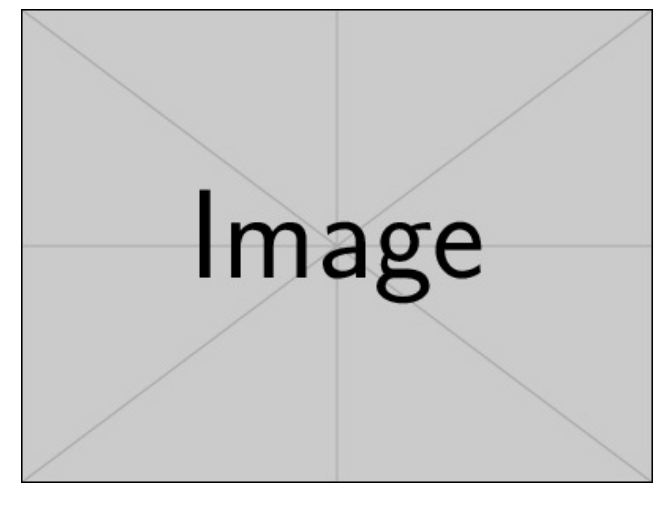
\includegraphics[width=0.20\textwidth,height=8.0mm]{figures/sample_image.png}}
%\lhead{{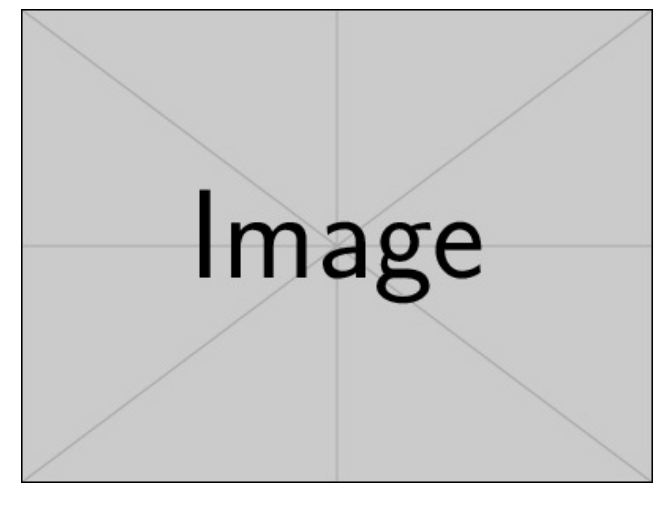
\includegraphics[width=0.20\textwidth,height=8.0mm]{figures/sample_image.png}}}

% Increase indentation in lists
\newlist{mydescription}{description}{1}
\setlist[mydescription,1]{labelindent=2em, leftmargin=2em}

%----------------CHAPTER------------------------------%
\titleformat{\chapter}[display]% shape
{\huge\bfseries}% format
{% label
    \makebox[50pt][l]{%
        \raisebox{0pt}[0pt][0pt]{%
            \textcolor{black!50}{\fontsize{100pt}{100pt}\selectfont\thechapter}%
        }% /raisebox
    }% /makebox
}% label
{0pt}% sep
{}% before-code
\makeatletter
\renewcommand\tableofcontents{%
    \par\par\textbf{\huge\contentsname}\par\par\par
    \@mkboth{\MakeUppercase\contentsname}{\MakeUppercase\contentsname}%
    \@starttoc{toc}%
}
\titlespacing{\chapter}{0pt}{20pt}{8pt}
\titlespacing{\section}{0pt}{0pt}{0pt}

\BeforeBeginEnvironment{figure}{\vskip 0ex}
\AfterEndEnvironment{figure}{\vskip 0ex}

\captionsetup{
    font=small,        % Small font size for captions
    labelfont=bf,      % Bold label (e.g., "Figure 1:")
    labelsep=colon,    % Separator between label and caption text
    justification=raggedright,  % Left-aligned text (or use 'justified')
    singlelinecheck=false        % Do not center single-line captions
}

%--------------------------------------%

% Fix for the "Contents" title indentation
\makeatletter
\renewcommand\tableofcontents{%
    \chapter*{\contentsname}% Custom alignment for the contents title
    \@starttoc{toc}% Generate the table of contents
}
\makeatother


\definecolor{dkgreen}{rgb}{0,0.6,0}
\definecolor{gray}{rgb}{0.5,0.5,0.5}
\definecolor{mauve}{rgb}{0.58,0,0.82}

% Settings for the 'listings' package to format Python code
% - frame=tb: Adds a top and bottom frame around the code block
% - language=python: Specifies that the code is Python
% - aboveskip/belowskip: Space above and below the code block (3mm)
% - showstringspaces=false: Hides underscores for spaces in strings
% - columns=flexible: Adjusts character spacing to fit the content
% - basicstyle={\small\ttfamily}: Sets the font style (small, monospaced)
% - numbers=none: Disables line numbers (can be 'left' or 'right' to show them)
% - numberstyle=\tiny\color{gray}: Styling for line numbers (if enabled)
% - keywordstyle=\color{blue}: Color for keywords (blue)
% - commentstyle=\color{dkgreen}: Color for comments (dark green)
% - stringstyle=\color{mauve}: Color for strings (mauve)
% - breaklines=true: Enables automatic line breaking
% - breakatwhitespace=true: Breaks lines at white space if necessary
% - tabsize=3: Sets tab width to 4 spaces
\lstset{frame=tb,
    language=python,
    aboveskip=3mm,
    belowskip=3mm,
    showstringspaces=false,
    columns=flexible,
    basicstyle={\small\ttfamily},
    numbers=none,
    numberstyle=\tiny\color{gray},
    keywordstyle=\color{blue},
    commentstyle=\color{dkgreen},
    stringstyle=\color{mauve},
    breaklines=true,
    breakatwhitespace=true,
    tabsize=4
}


% Force English titles for the ToC, LoF, and LoT
\renewcommand{\contentsname}{Table of Contents}
\renewcommand{\listfigurename}{List of Figures}
\renewcommand{\listtablename}{List of Tables}

% Remove "Chapter" from the chapter mark
\renewcommand{\chaptermark}[1]{\markboth{\thechapter\ #1}{}}

% Remove section numbering from the section mark
\renewcommand{\sectionmark}[1]{\markright{#1}}

% Define the custom header
% Define the custom page number style in the footer
\fancypagestyle{customHeaderFooter}{  % Use the 'customHeaderFooter' style for pages with no header
    \fancyhf{}  % Clear all headers and footers
    % Make the header semitransparent using TikZ
    \fancyhead[L]{%
        \begin{tikzpicture}[baseline=(current bounding box.south)]
            \node[opacity=0.65] {\leftmark};  % Chapter name on the left with transparency
        \end{tikzpicture}
    }
    
    \fancyhead[R]{%
        \begin{tikzpicture}[baseline=(current bounding box.south)]
            \node[opacity=0.45] {\rightmark};  % Section name on the right with transparency
        \end{tikzpicture}
    }

    \fancyfoot[R]{%
        \tikz[baseline=(X.base)] \node[fill=gray!20, minimum width=1cm, minimum height=2cm, text height=1.5ex, text depth=.25ex] (X) {\thepage};  % Custom right-aligned vertical box
    }
    \renewcommand{\headrulewidth}{0.6pt}  % Enable a header rule line
    \renewcommand{\footrulewidth}{0pt}  % Remove footer rule (if any)
}

% Prevent large white spaces by not stretching content
\raggedbottom

% Float behavior adjustment
\renewcommand{\topfraction}{0.7}     % Max fraction of the top page for floats
\renewcommand{\bottomfraction}{0.7}  % Max fraction of the bottom page for floats
\renewcommand{\textfraction}{0.2}    % Min fraction of page that must be filled with text
\renewcommand{\floatpagefraction}{0.6} % Min fraction of float page that must be filled

% Adjust spacing between floats and text
\setlength{\textfloatsep}{12pt plus 1.0pt minus 2.0pt}
\setlength{\floatsep}{12pt plus 1.0pt minus 2.0pt}
\setlength{\intextsep}{12pt plus 1.0pt minus 2.0pt}

% To create an icon from an image
\newcommand{\icon}[1]{\includegraphics[height=18pt]{#1}}
